\chapter{Análisis}
En este capítulo se aborda la fase de análisis de los distintos requerimientos  del sistema para cumplir con los objetivos del proyecto. Tanto los acertijos, las soluciones propuestas a ellos y la puntuación de cada solución son datos que son introducidos por los usuarios. El sistema tiene que ser capaz de poder permitir esa interacción de una manera sencilla e intuitiva.

En primer lugar se abordarán las cuestiones relativas al funcionamiento de la aplicación y, a partir de ahí, se definirá la arquitectura mediante la cual la aplicación podrá desarrollarse.

Una vez definida la arquitectura, se hará una búsqueda exhaustiva de las distintas tecnologías existentes que ayuden a cumplir los requisitos específicos de cada módulo que la forma, así pues se justificará la elección de la tecnología más adecuada para el desarrollo de la aplicación.

Por último, abordaremos el despliegue de la aplicación. Una vez más, se procederá a hacer una búsqueda exhaustiva de las distintas tecnologías que permitirán el despliegue en la nube de cada uno de nuestros módulos diferenciados. Una vez estén definidas, se procederá a la elección de aquella alternativa que nos solucione y complete nuestros requisitos.

\section{Requisitos de la aplicación}

La aplicación se presentará al usuario como una web actual en la que habrá que introducir usuario y contraseña para acceder. 

Desde el punto de vista del usuario, una vez dentro de la aplicación se presentarán todos los acertijos del sistema, pues el objetivo principal es que el usuario comience a interactuar. Por ello, es fundamental que en cualquier momento el usuario pueda:

\begin{itemize}
    \item Proponer un acertijo para compartir con los demás usuarios.
    \item Acceder a sus acertijos para consultar su estado.
    \item Puntuar las soluciones propuestas a sus acertijos.
    \item Proponer soluciones a cualquier acertijo del sistema.
\end{itemize}

Desde el punto de vista del sistema, para conseguir materializar las funciones básicas a llevar a cabo por un usuario y, aún más importante, la gestión de las mismas por un servicio que sea adaptable a cualquier tipo de interfaz, será necesario el desarrollo de una API REST, que actúe como intermediario entre la interfaz y la base de datos.

Aún dentro del sistema, es necesario el almacenamiento de toda esa información que será usada por el usuario continuamente en una base de datos intuitiva, actual y sencilla de manejar.


\section{Arquitectura Modelo-Vista-Controlador}
\label{sec::arquitecturaMVC}
Una vez definido el funcionamiento general de la aplicación, se pueden distinguir 3 bloques o módulos bien diferenciados:

\begin{itemize}
    \item Interfaz o front-end
    \item API REST
    \item Base de datos
\end{itemize}
 
 La arquitectura \textit{MVC} (Modelo Vista Controlador) es la más adecuada para el desarrollo de este proyecto, ya que nos permite hacer una distinción de tres bloques independientes que colaborarán entre sí para formar nuestra aplicación\cite{mvc2}\cite{mvc3}. Esta arquitectura distingue los bloques\cite{mvc1}:
 
 \begin{itemize}
    \item \textbf{Vista}. En este bloque es donde se representan los datos con los que el sistema operará. En nuestro caso, es nuestra interfaz.
    \item \textbf{Controlador}. Este bloque será el responsable de responder a los distintos eventos en los que se solicite algún tipo de consulta al modelo, o los que se necesite un transporte de información desde el modelo a la interfaz o viceversa. En nuestro caso, será nuestra API.
    \item \textbf{Modelo}. En este bloque se definirá el tipo de datos y su almacenamiento lógico. En nuestro caso, será nuestra base de datos.
\end{itemize}
\begin{figure}[htbp]
    \centerline{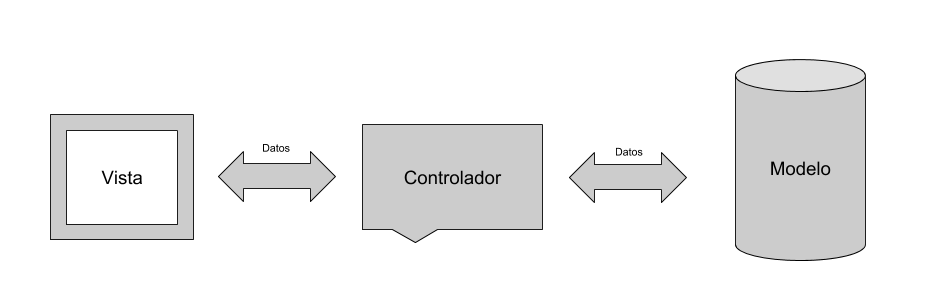
\includegraphics[width=11cm]{figuras/mvc.png}}
    \caption{Arquitectua Modelo-Vista-Controlador}
    \label{fig::mvc}
\end{figure}
Cada bloque de nuestra arquitectura se abordará de manera independiente, teniendo muy en cuenta, que éstos, una vez definidos y desarrollados, tendrán que estar conectados para así permitir el flujo de información correspondiente a los eventos por parte de los requisitos del usuario. 

En la imagen \ref{fig::mvc} se pueden contemplar los tres bloques que forman la arquitectura MVC.


 
\section{Tecnologías a emplear}

Comenzaremos definiendo las posibles tecnologías que encontramos para desarrollar cada uno de los bloques de nuestra aplicación. Para escoger las tecnologías a emplear, nos basaremos en los requerimientos de la aplicación y nuestra propia intuición como desarrolladores.

\subsection{Tecnologías de desarrollo}

Inicialmente se hará una búsqueda de las distintas tecnologías para el desarrollo del bloque, se compararán y se decidirá cual de ellas es la escogida y el por qué.

\subsubsection{Modelo - Base de Datos}

En el mercado podemos encontrar dos tipos distintos de bases de datos: relacionales y no relacionales\cite{tipobd}. 

Para el desarrollo de nuestro proyecto, estamos buscando una base de datos que sea intuitiva y sencilla de administrar. Es fundamental encontrar una base de datos que administre eficientemente unos datos de una manera distinta a la visión de "tabla" que nos ofrecen las bases de datos relacionales. Es por ello que se ha escogido una base de datos \textbf{no relacional} para el almacenamiento de los datos de la aplicación.

Dentro de las bases de datos no relacionales encontramos distintos tipos:

\begin{itemize}
    \item Bases de datos documentales
    \item Bases de datos en grafo
    \item Bases de datos clave/valor
    \item Bases de datos multivalor
    \item Bases de datos orientadas a objetos
    \item Bases de datos tabular
    \item Bases de datos de arrays
\end{itemize}

Ante esta abrumadora lista de alternativas, el tutor recomendó que se usaran\textbf{ bases de datos orientadas en grafos}. Este tipo no relacional de bases de datos está en auge y se planea que para un futuro no muy lejano sea el tipo de base de datos más usado\cite{bdnorel1}\cite{bdnorel2}. 

Dentro de las bases de datos basadas en grafos se pueden encontrar dos de las más solicitadas:

\begin{itemize}
    \item neo4j\footnote{https://neo4j.com/}
    \item titan\footnote{http://titan.thinkaurelius.com/}
\end{itemize}


Para nuestra base de datos buscamos la sencillez, la simplicidad y el uso de un único proceso que actúe como servidor e interfaz gráfica de una base de datos intuitiva. La facilidad de instalación y manejo de \textbf{neo4j} la han convertido en la candidata ideal para nuestra aplicación.  Además es importante tener en cuenta la facilidad a la hora de conectar con cualquier API y escalar conforme el tamaño de la base de datos aumente, la posibilidad de hacer copias de seguridad en local y, sobre todo, la aparición de \textit{cypher} como lenguaje de consulta\cite{neovstitan}.

Gracias al inmejorable\textit{online training} y la perfecta descripción de la documentación oficial de neo4j\footnote{https://neo4j.com/graphacademy/online-training/} el aprendizaje de este concepto nuevo de bases de datos y su lenguaje de consulta ha sido un proceso sencillo de llevar a cabo.

El uso de Cypher\footnote{https://neo4j.com/developer/cypher-query-language/} como lenguaje de consulta ha facilitado notablemente la elección de esta base de datos, pues gracias a éste solamente tenemos que tener en cuenta nodos y relaciones que hay entre ellos. Con una serie de órdenes simples podemos gestionar excesivamente rápida e intuitivamente toda la información que necesitemos para el funcionamiento de nuestra aplicación.

\subsubsection{Controlador - API REST}

Para que nuestra API sea sencilla de implementar, usando un lenguaje simple, de alto nivel y con un inicio sencillo a la hora del aprendizaje, libre y con una documentación extensa y infinitud de librerías podemos escoger, podemos distinguir varios lenguajes actuales y de los más utilizados para la creación de servicios rest\cite{apirest1}\cite{apirest2}\cite{apirest3}:

\begin{itemize}
    \item Javascript - Nodejs
    \item Python
    \item Java 
    \item PHP
    \item Ruby
\end{itemize}

Ante estas alternativas, todas son válidas y reúnen la documentación necesaria para desarrollar el proyecto. Es por ello, por lo que para tomar esta decisión se tendrá en cuenta la formación  práctica durante el Grado en Ingeniería Informática de la UGR. En esta línea, se ha seleccionado \textbf{\textit{python} }, pues es un lenguaje en el que, desde el punto de vista personal, se tiene menos soltura en comparación con otros, con lo que optar por desarrollar el proyecto en este lenguaje supone una gran oportunidad para desarrollar nuevas aptitudes y habilidades.

Además, \textit{python} es un lenguaje que se está convirtiendo en uno de los más utilizados en la plataforma líder en software libre GitHub\footnote{https://octoverse.github.com/}, con lo que además se abordaría uno de los requisitos a tener en cuenta en el desarrollo del proyecto: la utilización de tecnologías actuales.

Una vez decidido el lenguaje, existen dos alternativas bien diferenciadas a la hora de crear un servicio web en \textit{python}:

\begin{itemize}
    \item Flask\footnote{http://flask.pocoo.org/}
    \item Django\footnote{https://www.djangoproject.com/}
\end{itemize}

Una vez estudiadas las características principales de cada alternativa\cite{flaskvsdjango1} , y puesto que nuestra aplicación necesitará de un gestor ligero que contenga solamente métodos que se llamarán desde nuestra interfaz e interactúen con la base de datos, descartamos la opción de usar Django, pues éste es demasiado pesado y tiene añadida la gran dificultad de comprender la estructura con la que funciona. Est es justo lo contrario que Flask, una herramienta simple de entender y que con poco tiempo de estudio se es apto para desarrollar una API que cumpla los requisitos de nuestra aplicación. 

Nuestra API, por lo tanto estará escrita en \textit{\textbf{Python}} y se usará el framework \textbf{Flask}.

\subsubsection{Vista - Interfaz}
\label{sec::analisis_vistaInterfaz}
Existen infinidad de frameworks y lenguajes a la hora de desarrollar una interfaz web. Con la idea de querer implementar una interfaz que sea interactiva y ligera, se busca un lenguaje que permita el desarrollo de una web básica, con un ligero aspecto de red social, ya que se busca en todo momento, que el usuario se enganche a la aplicación. Para ello es fundamental el uso de una interfaz fácil de utilizar.

Para la búsqueda de este framework se ha tenido muy en cuenta, primero que el lenguaje que lo soporte sea sencillo, rápido, muy bien documentado, con muchas librerías adicionales, soportado en el máximo de navegadores y, que se puedan llegar a cumplir todos los requerimientos que la interfaz necesita, como por ejemplo, la capacidad de realizar peticiones HTTP a nuestra API o controlador.

Todos estos motivos nos hacen decantarnos por \textbf{javascript} como el lenguaje principal para esta interfaz. Además, este lenguaje nos proporciona diferentes frameworks para el desarrollo de nuestra interfaz\cite{framework}:

\begin{itemize}
    \item AngularJS\footnote{https://angularjs.org/}
    \item ReactJS\footnote{https://reactjs.org/}
    \item VueJS\footnote{https://vuejs.org/}
    \item EmberJS\footnote{https://www.emberjs.com/}
    \item Aurelia\footnote{https://aurelia.io/}
\end{itemize}

Al estudiar en profundidad las características de cada uno\cite{framework2}, se ha escogido \textbf{ReactJS}. Este framework tiene la gran ventaja de que está siendo el más usado hoy en día por plataformas tales como Instagram o Facebook. Es más, ReactJS es una librería desarrollada por Facebook, lo cual quiere decir que tiene un soporte que garantiza una larga vida a largo plazo.

ReactJS tiene como inconveniente la curva de aprendizaje pues puede ser un poco complicado al principio. Sin embargo, gracias a la buena documentación y a los tutoriales a los que podemos acceder a través de la web oficial, y sobre todo, gracias a la gran comunidad que está apareciendo sobre este framework, se garantiza la alta probabilidad de alcanzar los objetivos en el período de tiempo estimado.

Un framework como ReactJS está basado en la creación de componentes y su reutilización. Esto es de gran ayuda pues en nuestra aplicación aparecerán distintos datos en pantalla, todos esto apoyados en una misma estructura visual que se mantendrá fija salvo, obviamente, que se solicite la muestra de información específica.

\subsection{Tecnologías de despliegue}

Una vez definidas las tecnologías que se usarán para cada bloque de la arquitectura modelo vista controlador, el objetivo será alojar cada uno de éstos en la nube y conectarlos entre sí. 

Existen distintos formas de desplegar en la nube\cite{cloud}\cite{cloud2}\cite{cloud3}\cite{cloud4}:

\begin{itemize}
    \item Software como Servicio o \textbf{SaaS}. Es un modelo donde el soporte hardware de la infraestructura está gestionado por el proveedor del servicio. El servicio y el software están ya definidos. Los datos los tiene almacenados el  hardware del proveedor del servicio. Un ejemplo de SaaS sería: Dropbox o Gmail.
    \item Plataforma como Servicio o \textbf{PaaS}. Un PaaS proporciona un entorno cloud donde se puede crear una aplicación, es decir, podemos definir qué tipo de servicio queremos implementar. Por la parte hardware, es el proveedor el que se encarga de los recursos de infraestructura dedicados a ese servicio. Un PaaS está justo encima de la capa de infraestructura, nos proporciona la posibilidad de crear un servicio sin tener que preocuparnos por los recursos hardware que se necesitarán para el correcto funcionamiento del servicio.
    \item Infraestructura como Servicio o \textbf{IaaS}. Un IaaS es un modelo en el que tenemos la libertad de implementar cualquier servicio, pero con la posibilidad de definir una infraestructura que sustente ese servicio. Se deben de proveer los recursos necesarios para el arranque del servicio.
\end{itemize}

En esta aplicación se busca la velocidad y la sencillez, sin entrar demasiado en la definición de los recursos hardware a utilizar. Es por ello que un IaaS retrasaría bastante el desarrollo de la aplicación, pues no está contemplado la posibilidad de definir una infraestructura hardware para este proyecto.

Para la realización de este proyecto se usarán \textbf{PaaS} y \textbf{SaaS}.

\subsubsection{Vista - Interfaz}

En el mercado nos podemos encontrar diversos PaaS donde poder alojar y desplegar nuestro servicio, con infinidad de posibilidades para desplegar. En nuestro caso, para  el despliegue de la interfaz se ha usado \textbf{Heroku}\footnote{https://dashboard.heroku.com/}.

Esta plataforma nos ofrece la posibilidad de enlazar nuestro repositorio en GitHub con Heroku y automatizar proceso de despliegue con un simple click. Es por ello que esta plataforma es la idónea, pues en este proyecto se busca exhaustivamente la automatización de procesos como el despliegue y la verificación.

\subsubsection{Controlador - API}

Destacando otra vez la facilidad y automatización del despliegue. \textbf{Zeit}\footnote{https://zeit.co/now} nos ofrece una herramienta llamada \textbf{Now} que nos hace increíblemente cómodo el despliegue de nuestra API.

Zeit nos permite desplegar nuestra API de manera automática, con solo un comando: \textit{now}. Adicionalmente se necesitaría un archivo en el que se especifique el entorno de nuestra aplicación, esto es, por ejemplo:

\begin{itemize}
    \item Lenguaje utilizado.
    \item Librerías a instalar que utiliza el servicio.
    \item Puerto por el que se transmitirá información. En nuestro caso, solamente realizaremos peticiones HTTP, por lo que el puerto será el 80.
    \item Localización de nuestro ejecutable y comando para ejecutarlo.
\end{itemize}

\subsubsection{Modelo - Base de datos basada en grafos}

En este apartado no se encuentran tantas alternativas para el despliegue en la nube de una base de datos basada en grafos. La propia documentación de neo4j (nuestra base de datos escogida) nos recomienda \textbf{GrapheneDB}\footnote{https://www.graphenedb.com/} como SaaS donde almacenar nuestra base de datos.

Es una decisión rotundamente acertada. Es muy sencillo el uso para la creación de una base de datos basada en grafos en dicha plataforma.